\chapter{Application context}\label{chp:2}

\minitoc

\clearpage

One of the most recent policy responses made to address environmental issues in Europe is the European Partnership for the Assessment of Risks from Chemicals (PARC) \citep{PARC}. This partnership involves 28 different countries. This new project was positively evaluated by the European Commission in January 2022 and started on the 1st of May 2022. The main objectives of PARC are to promote European cooperation, advance research, increase knowledge of chemical risk assessment and train relevant methodological skills. Close cooperation between authorities and researchers will facilitate the translation of research results into regulatory practise. \\
The French Agency for Food, Environmental and Occupational Health and Safety (ANSES\footnote{Agence nationale de sécurité sanitaire, de l'alimentation, de l'environnement et du travail}) is not only the main French actor in this partnership, but also the coordinator of the whole partnership. This manuscript is the result of a mission funded by ANSES and aimed at supporting the Agency in its mission on French territory. In order to better understand the topics covered in this manuscript, it is necessary to have a presentation of the Agency and its tasks, as well as the means at its disposal to carry out some of its tasks. This chapter describes the overall context and the specific issues arising from the characteristics of the data used. The chapter is structured as follows: In \ref{chp:2:1} we introduce ANSES, in \ref{chp:2:2} we explain the task of pesticide monitoring, in \ref{chp:2:3} we focus on the characteristics of the pesticide measures, in \ref{chp:2:4} we describe other sources of information of interest and in \ref{chp:2:5} we define the intended objectives.

\section{ANSES presentation}\label{chp:2:1}

ANSES was created in 2010 from the merger of the French Food Safety (AFSSA) and the French Agency for Environmental and Occupational Health Safety (AFSSET). It is a public administrative establishment under the authority of the Ministries of Health, the Environment, Agriculture, Labour and Consumer Affairs.

\subsection{Missions} 

The ANSES agency has many missions. Let us introduce the most important ones.
\begin{itemize}
\item \textbf{Research activities:} The Agency contributes to the advancement of scientific knowledge on the exposure of humans, animals, plants and the environment to various hazards and risks and has the mission to improve their monitoring. The research topics focus on three areas: Animal Health and Welfare, Plant Health and Food Safety. ANSES is also involved in the development of new analytical methods and detection techniques to identify pathogens and contaminants, whether in the natural environment or in the production chain. This mission also groups health surveillance and alert activities. The Agency participates in epidemiological surveillance platforms for animal health, plant health and food chain safety. Under this mandate, ANSES is also in charge of coordinating five different surveillance systems covering: toxicovigilance, food supplement surveillance, phytopharmacovigilance, which is further explored in \ref{chp:2:2}, veterinary pharmacovigilance and occupational disease surveillance and prevention. 
\item \textbf{Risk assessment:} ANSES responds to society's questions on potential risks arising from the consumption of food, the use of certain products or technologies, professional activities or the pollution of various environmental compartments (e.g. air, water or soil). Given the complex risks, the Agency has developed a working methodology that brings together many disciplines to provide the most comprehensive response possible. The risk and efficacy assessment of veterinary medicinal products and phytopharmaceuticals for human and animal health and for the environment also falls within the Agency's remit. The aim is to define measures for dealing with such risks. The ANSES is responsible in particular for issuing sales authorisations for such products and thus also has the power to withdraw products at national level \citep{ansesdec}. 
\item \textbf{Public and environmental protection:} ANSES makes recommendations to support public debates and decisions. Its activities contribute to the implementation of effective preventive and protective measures on various societal issues such as health, biodiversity and ethics. It also provides the public with access to reliable, independent and multidisciplinary scientific information. The Agency's mission is to respond flexibly to already known or emerging, short- or long-term sanitary risks. In other words, the aim is to identify any emerging signals as quickly as possible and make recommendations, even in times of crisis with scientific uncertainty. The task is then to reduce the level of uncertainty as much as possible. The recommendations are based on all available knowledge, whether generated by the agency itself or by its partners. 
\end{itemize}

\subsection{Means of action}

The ANSES has the means to carry out and fund research in collaboration with the French and international scientific communities. It has 9 laboratories distributed among its 16 sites on French territory (including overseas departments). The research carried out in these facilities addresses the complex interactions between the environment, human health and animal health. The aim is to anticipate the emergence of zoonoses or animal diseases that could have an economic impact and to combat antibiotic resistance. Specifically, the main directions of this research are:
\begin{itemize}
\item To learn the characteristics of pathogens (such as fungi, bacteria, viruses or parasites), macro organisms (such as insect pests or invasive plants) and chemical contaminants. 
\item To detect them using state-of-the-art analytical methods.
\item To monitor them using powerful epidemiological methods.
\item To understand the impact of animal husbandry on animal welfare and health.
\item To develop useful knowledge for the development of new treatments and vaccines to prevent and control animal and plant diseases. 
\end{itemize} 
The 9 laboratories have been designated as reference laboratories for pathogen research under more than 100 national and international mandates \citep{ANSESLABS}.

In addition to its research activities, ANSES is also at the centre of a network of partners. Given the scope of the areas it covers, the Agency does not have the resources to collect data on all the topics it is tasked with. Therefore, for each topic, it holds discussions with other organisations that are likely to be able to provide interesting sources of information. For example, each monitoring system coordinated by the Agency mobilises a different set of partners. We will see the different datasets that these partners bring in Sections \ref{chp:2:3} and \ref{chp:2:4}.

\subsection{Specific organisation}

Many national agencies are counterparts of ANSES. They all participate in the PARC partnership. Each of them shares data collected at national level, enabling research studies at European level. However, each agency is dependent on the network that collected the data it stores and on the internal policies of the country to which it belongs. This leads to heterogeneity on different topics and at different levels. \\
For example, internal policies influence the list of products monitored, and some substances are not tested in certain countries because they are not even approved for sale. This leads to a patchwork of different substances lists at the European level, as shown in \cite{Baran2022}. A certain heterogeneity can also be observed at the national level. For example, in France it has been established that data on drinking water quality should be collected at regional level, see for example \cite{Baran2022}. Each regional agency is responsible for the quality of the data it shares with ANSES. We will see the impact of this organisation on the data in Section \ref{chp:2:3}. \\
The structure of the monitoring system is thus country-specific. This is especially true for the pesticide monitoring system, which we will focus on below.

\section{Pesticides monitoring mission}\label{chp:2:2}

Although the term risk is often confused with hazard in common usage, they do not have the same definition. A \textbf{health hazard} is the inherent ability of a substance or organism to cause adverse health effects. \textbf{Exposure} is the specific situation in which people are confronted with a health hazard. Exposure can be characterised by the following questions:
\begin{itemize}
\item What was the degree or intensity of exposure?
\item How long and how regularly does the exposure occur? 
\item In what way does the exposure occur? (E.g. skin contact, ingestion, etc.)
\end{itemize}
A \textbf{health risk} occurs when one is exposed to a health hazard. It is defined as the probability of the occurrence of adverse effects on human health. It can take many forms, such as infection, poisoning or chronic disease (such as diabetes or asthma). The outcome depends on the characteristics of the exposure and the characteristics (such as age or immunity) of the animal, human or plant population studied.

The ANSES has the task of investigating and monitoring health risks caused by various factors. In particular, the agency is tasked with monitoring health risks related to chemical substances, as pesticides. The pesticide monitoring mandate can be formally defined as a surveillance system that collects and evaluates data on phytopharmaceuticals (pesticides). It can also be referred to as phytopharmacovigilance. The aim is to detect adverse effects associated with the use of these products as quickly as possible in order to protect the health of living organisms and ecosystems. The health hazards of pesticides are well referenced by the Agency and available in the AGRITOX database \citep{AGRITOX}. Depending on the population concerned by the monitoring, different types of exposures can be distinguished. In the following, two concrete cases are presented to illustrate the variability of exposures that can be observed in practice. The first case concerns the monitoring of the health risk of professional farmers. They are regularly exposed to the pesticides they use. The exposure is then of long duration and the likely routes through which they could come into contact with the substance would be inhalation or skin contact. The second case is about monitoring the health risk to aquatic fauna. Exposure to pesticides may result from the effects of water run-off after pesticide application, which could lead to dispersal into the river system in the area. As the pesticide is in the same environment as the aquatic fauna, it could come into direct contact with them and cause adverse effects (acute or chronic). It should be noted that diffusion and thus exposure both depend on external factors, independent of the intrinsic properties of the substance. One example would be the meteorological conditions during the study period. Another example would be the consideration of environmental characteristics that are likely to influence the diffusion of the substance. For example, the diffusion of a chemical product in a river system could be influenced by the composition of the river bed or the width of the river. Therefore, it would be interesting to study exposure in regions where these characteristics are fixed. The hydro-ecoregions (HER) take into account such characteristics and would provide a coherent additional analytical tool for the river system example.           

ANSES does not itself collect the data it needs to fulfil its phytoharmacovigilance mandate. It relies on its partner network to obtain datasets of interest. The decision to add a new source of information first requires a discussion on the coherence of the use of this source of information to provide an answer to the problem under investigation. For phytopharmacovigilance, the following information is of interest: 
\begin{enumerate}
\item contamination of the environment - air, water, soil, food and drinking water - by residues including metabolites of pesticides.
\item exposure, impregnation and effects on living organisms and ecosystems as a whole: humans, livestock and wildlife, crops, flora, etc. Resistance phenomena in organisms targeted by these molecules: Pathogens, weeds, insects.
\end{enumerate}
This leads to the collection of spatio-temporal information. The datasets that provide information on pesticide concentrations and use are presented in detail in Section \ref{chp:2:3}.

\section{Pesticide measurement data}\label{chp:2:3}

There are two types of measurements: direct measurements, which are essentially stations that measure the exact concentration of a substance in a particular environment, and indirect measurements, which give indications of the use of a substance.

\subsection{Direct measurement characteristics}

Access to direct measurement data is often public and data can be accessed from various portals depending on the monitored environment. These include: the Naiades portal for surface water quality \citep{Naiade2}, the Ades portal for underground water quality \citep{Ades}, the Geodair portal for air quality \citep{Geodair}.
 
This part examines the characteristics of pesticides measured directly by sampling stations. The following characteristics are not present systematically, but are very common when it comes to concentration measurements.

\subsubsection{Chemical precision limits in measurements}

The first specificity of concentration measurement arises from the problem of measuring a chemical substance in a sample. In applied chemistry, every measuring device is characterised by two types of limit values: 
\begin{itemize}
    \item The limit of detection (LOD): This is the smallest concentration value in a sample that can be distinguished from zero with sufficient certainty.
    \item The limit of quantification (LOQ): This is the smallest concentration value of a substance in a sample that can be measured with  sufficient certainty. 
\end{itemize}
These limits are determined by the sensors with which the sampling station is equipped. It happens that geographical areas are covered by stations that do not have the same equipment. In this case, there are several LOQ values among the samples taken in that area. In the case of surface waters, for example, the contracts for the selection of monitoring laboratories are awarded by the water agencies. These agencies, six in number, cover areas larger than the French administrative regions. Administrative regions can be partially included in the area covered by a water agency. This means that if the scale of an administrative region is taken as the basis for a study, this region may fall under the jurisdiction of two different water agencies and the measuring instruments may therefore be different. Furthermore, the same station may change its measuring equipment over time. Contracts for station equipment are renewed periodically, but renewal does not guarantee that the same equipment will be maintained. These two accuracy limits imply that the concentration data are left-censored. All these features are shown in Figure \ref{fig:cens_ex} where concentration values of the herbicide prosulfocarb are used to illustrate the censoring. Several methods have been developed to handle this type of data. We can cite the imputation of values to replace the LOQ values in the set of concentration values, the use of the maximum likelihood estimator or the Kaplan-Meier estimator (see \cite{Gillaizeau2020,Croghan2003MethodsOD}). In Chapter 4 we will show which method was chosen for this type of data in this thesis. 

\begin{figure}
    \centering
    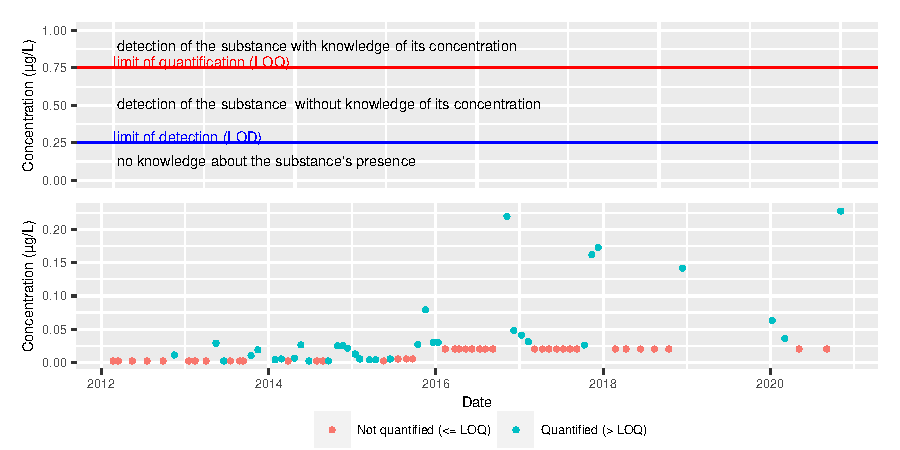
\includegraphics{Chap3/Cens_ex.pdf}
    \caption{Censorship illustration. The top Figure sums up the limits of measurements effects. The bottom Figure shows the consequences of censorship on the samples of a station located in the Centre-Val de Loire region. This station replaced its equipment in 2016, so the LOQ has changed.}
    \label{fig:cens_ex}
\end{figure}

\subsubsection{Irregular sampling}

The second feature is a direct consequence of Section \ref{chp:2:1}. We have already mentioned that each country has organised its own monitoring system in different ways. Some features are country-specific and have an impact on the raw data of the collected samples. In France, samples are not necessarily collected at regular intervals, as you can see in Figure \ref{fig:cens_ex}. No concentration data were collected in 2019. This is also the case for water monitoring data. This is a specificity of the French network, as this is not the case in all countries. For example, \cite{Zhang2008} states that sampling in surface waters is regularly carried out in China. Furthermore, \cite{Joergensen2008} states that this is also the case for groundwater monitoring systems in countries such as China, the Netherlands and South Korea. The South Korean monitoring system is even automatic. Every six hours a sample is taken and after analysis it is automatically stored on a central server. We would also like to point out that strategies other than regular sampling, such as grab sampling \citep{Novic2017}, could explain the irregular sampling rhythm in French surface waters. Grab sampling is about getting as accurate a picture as possible of surface water quality in a short time (and in a limited area). If the operations of grab samples and periodic monitoring operations of a station are recorded in the same database, irregular sampling may also occur.

\subsubsection{Spatio-temporal heterogeneity in sampling}

Another important feature mentioned in \cite{Baran2022} is the spatial and temporal heterogeneity of the records. This heterogeneity becomes clear when comparing measurements made in two different areas. Figure \ref{fig:het_sampspat} illustrates that the activity periods of stations in two different geographical zones differ. Figure \ref{fig:het_sampspat} also shows that the stations make very few measurements. The two groups have the same number of stations and yet group 2 has taken fewer measurements than group 1 over the same period of time.

\begin{figure}[htbp]
    \centering
    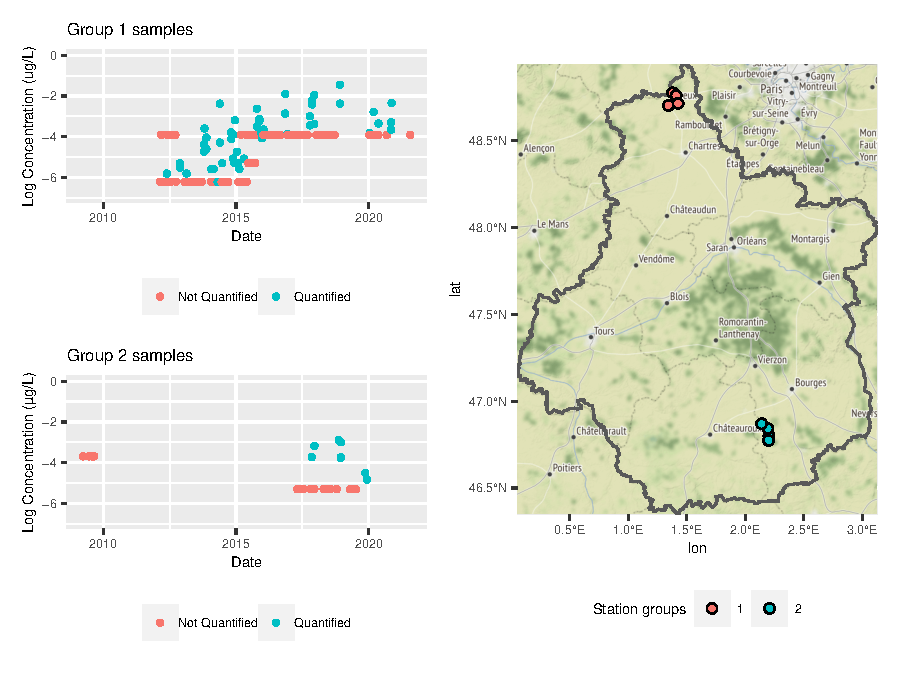
\includegraphics{figs/Chap3/Het_sampling.pdf}
    \caption{Spatial and temporal heterogeneity in sampling. The Figures on the left represent all the samples of two groups of stations. The map on the right shows the position of those groups. Concentration of prosulfocarb in surface waters are used for this illustration.}
    \label{fig:het_sampspat}
\end{figure}

This problem of heterogeneity persists even with two spatially adjacent stations. The measured values are not synchronous in time. In Figure \ref{fig:het_samp_ex} we see that it is difficult to compare the measurements of two existing stations. This would mean making strong assumptions about the temporal evolution of the concentrations. The stations sampled at non-overlapping time periods. One may notice that aggregating the data from the two stations results in a time series that is more evenly sampled over time. More details on this issue are provided in Section \ref{chp:2:4}.

\begin{figure}[htbp]
    \centering
    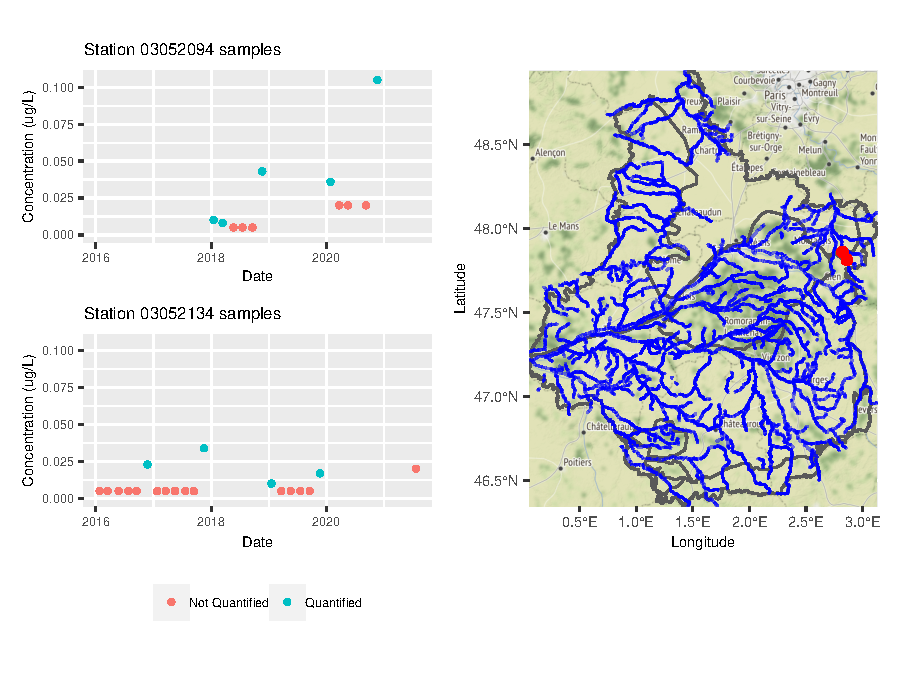
\includegraphics{figs/Chap3/Hetero_ex.pdf}
    \caption{Spatial and temporal heterogeneity in sampling. The Figures on the left represent all the samples of two neighbouring stations. The map on the right shows the position of those stations. Prosulfocarb concentration in surface waters is used for this illustration.}
    \label{fig:het_samp_ex}
\end{figure}

\subsubsection{Spatio-temporal heterogeneity in analytical results}

Figure \ref{fig:het_spa_ex} illustrates that in addition to the temporal heterogeneity caused by the different sampling rhythms of the stations, the spatio-temporal data are also not homogeneously distributed over the territory. The concentration values seem to differ completely depending on their spatial area of origin. Figure \ref{fig:het_spa_ex} also illustrates that the distribution of concentration values can change drastically over time. Looking at the samples of station 03189000, there is a breakpoint in the concentration values of the station just before the year 2015. The same is true for the year 2016 in Figure \ref{fig:cens_ex}. 
\begin{figure}[htbp]
    \centering
    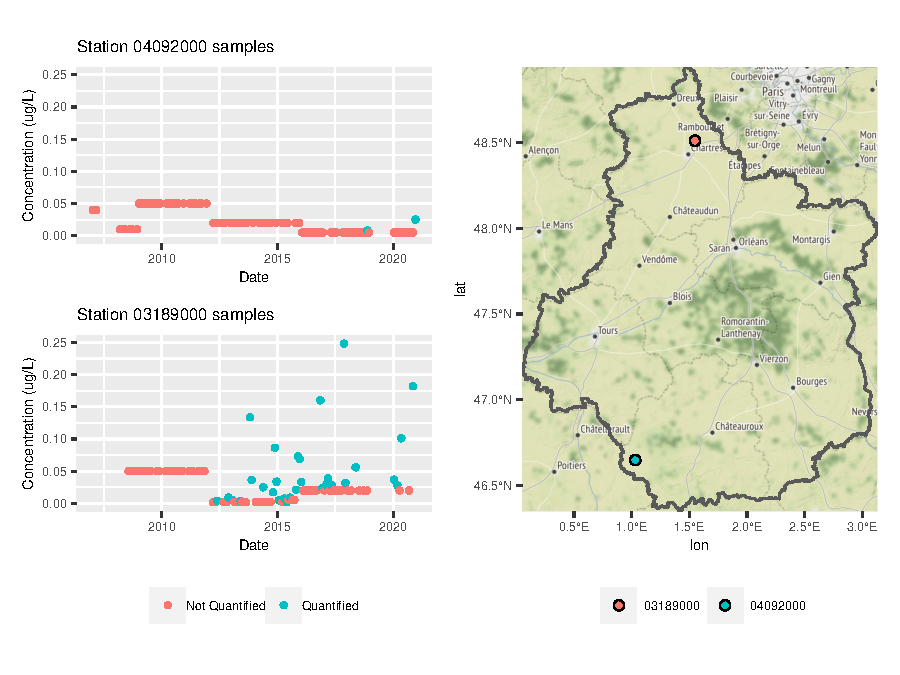
\includegraphics{figs/Chap3/Het_resC.pdf}
    \caption{Spatial and temporal heterogeneity in distribution. The Figures on the left represent all the samples of two stations. The map on the right shows the position of those stations. Prosulfocarb concentration in surface waters is used for this illustration.}
    \label{fig:het_spa_ex}
\end{figure}
This indicates that the use of a particular substance is not evenly distributed over the entire area. The spatio-temporal heterogeneity of concentration values can be easily explained by differences in agricultural practises depending on various factors related to professional habits and geological characteristics.

%\subsubsection{Spatio-temporal heterogeneity}

%Another main characteristics mentionned in \cite{Baran2022} is the spatio-temporal heterogeneity in the data-sets. Figure \ref{fig:het_samp_ex} shows the temporal heterogeneity. For two spatially neighbouring stations the measured values are not synchronous in time. It can also be seen that the stations take very few measurements and do not take the same number of measurements. In Figure \ref{fig:het_samp_ex} we see that it is complicated to compare the measurements of the two existing stations. It would imply making strong assumptions on the concentrations temporal evolution. The stations made samples in non-overlapping time periods. One may notice that aggregating the data from the two stations results in a time series that is more evenly sampled over time. More details on this issue are provided in Section \ref{chp:2:4}. 

\subsection{Indirect measurements information}

\subsubsection{Surveys on farming practises}

Additional indications of the presence of the substance are provided by surveys of agricultural practises. They are conducted by the Ministry of Agriculture in the form of a questionnaire and are used to describe and characterise how farmers work on their land. These surveys are very specific and focus only on certain types of crops. Three topics are addressed in the questionnaires. The first topic captures general information about the farm, such as a commitment to reducing pesticide use or agroecology. The second part of the questionnaire is designed to cover all technical operations on the farm plot. In other words, the department of the ministry examines the structure of the plantation, its preceding crops or its irrigation. Finally, the use of pesticides on the entire farm is also examined. The questionnaire addresses criteria such as the type and settings of the sprayer for the substance or the handling and protection of the user.
Figure \ref{fig:PK1} shows what kind of questions to expect in this survey \footnote{Document in French, full document in \cite{PK}}. In summary, surveys of agricultural practises provide much qualitative (rather than quantitative) information about the source of substance emissions. However, these surveys are conducted on an ad hoc basis and cover only certain types of crops. Only the results of the analyses by the statistical departments of the ministries of agriculture are publicly available \citep{PK2}, but not the raw data.

\begin{figure}[ht]
    \centering
    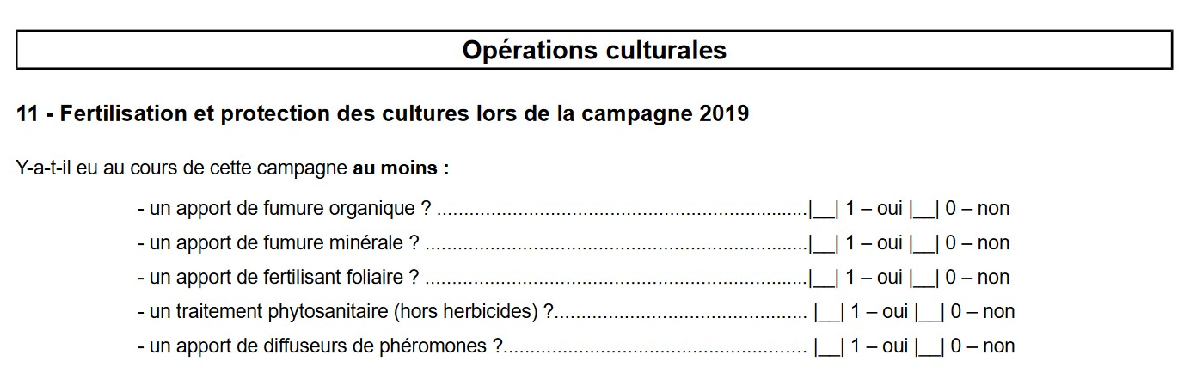
\includegraphics[scale=0.75]{figs/Chap3/PK1.pdf}
    \caption{Question extracted from the 2019 survey destined to viticulture. The question asked is about the fertilization and protection of the crops and the use of any phytosanitary product.}
    \label{fig:PK1}
\end{figure}

\subsubsection{Substances sales databank}

The use of a substance can also be seen indirectly in the sales data of plant protection products. The National Bank for the Sale of Pesticides by Authorized Distributors (NBSD) \cite{BNVD} lists and archives all such data. For reasons of anonymity, geographically fine resolution information is not available. The most precise resolution corresponds to postcodes. The same applies to the temporal resolution, which is no finer than the annual resolution. This dataset does not provide information on the location and date of use of the substance. A buyer may well be in a different place from the place where he used the substance he has just bought. Nevertheless, sales give a general indication of the intensity of use of a substance. A sudden increase in sales of a product, as shown in Table \ref{tab:bnvd}, may mean that use in that area is increasing.

\begin{table}[ht]
\centering
\begin{tabular}{rlllrr}
  \hline
 & Year & Department & Substance & Quantity sold (in kg) & Annual rank \\ 
  \hline
1 & 2008 & INDRE & 2,4-db & 27.00 & 155 \\ 
  2 & 2009 & INDRE & 2,4-db & 24.00 & 162 \\ 
  3 & 2010 & INDRE & 2,4-db & 24.00 & 166 \\ 
  4 & 2011 & INDRE & 2,4-db & 68.00 & 148 \\ 
  5 & 2012 & INDRE & 2,4-db & 7.00 & 195 \\ 
  6 & 2013 & INDRE & 2,4-db & 72.00 & 157 \\ 
  7 & 2014 & INDRE & 2,4-db & 120.00 & 125 \\ 
  8 & 2015 & INDRE & 2,4-db & 84.00 & 146 \\ 
  9 & 2016 & INDRE & 2,4-db & 195.00 & 108 \\ 
  10 & 2017 & INDRE & 2,4-db & 348.00 & 105 \\ 
   \hline
\end{tabular}
   \caption{Annual sales of the weed killer 2,4-db in the Indre department. The last column indicates the national annual rank of the substance sales.}\label{tab:bnvd}
\end{table}

\subsubsection{Crops cartography}

Specific pest species can be observed for each crop type. Mapping the crop types in an area can therefore give a first idea of the areas and application periods of the substance to be monitored. Some of this information is available in the graphical land register (GLR) \citep{RPG}. This database corresponds to the application forms used by farmers to obtain grants from the Common Agricultural Policy of the European Union (CAP). To be eligible for these subsidies, the crops grown on the plots must be declared. This dataset is partial information, as it is not compulsory to apply for the funds from CAP. Therefore, the owners of the cultivated areas who have not applied for aid are not included in the database. Furthermore, this register is renewed every year. It is possible that the information for certain parcels is not included in all annual editions of the GLR. As an example, cultivation maps for barley and wheat are shown in Figure \ref{fig:crops} of the Annex \ref{section:crops}.

%\footnote{Available at : \url{https://www.data.gouv.fr/fr/datasets/registre-parcellaire-graphique-rpg-contours-des-parcelles-et-ilots-culturaux-et-leur-groupe-de-cultures-majoritaire/}.}

\subsubsection{Adverse effects databases}

The final example of data that can provide clues to the use of a substance are the databases used to monitor possible adverse events. They consist of medical registers that provide information on human and animal health. 
For human health, several sources of information can be cited: 
\begin{itemize}
\item The Phytattitude network was developed by the Mutual Agricultural Health Insurers (MSAs). It is a network where any professional who comes into contact with phytosanitary products can indicate if they have any health problems. This organisation collects data through spontaneous reports from agricultural actors or during planned visits by nurses or doctors.
\item The medical-administrative databases of the MSA. They collect information on reimbursement for farmers' health care.
\item The poison control centres are involved in monitoring adverse effects. They provide information on toxicovigilance for the whole population. Much information about acute health problems comes through these information channels.
\item The National network of vigilance and prevention of professional pathologies (RNV3P), whose task is to identify emerging or re-emerging occupational health risks, is a good source for chronic health problems.
\item The AGRICAN cohort (AGRIculture and CANcer) of the François Baclesse Centre is used to measure the health status of the agricultural population compared to the general population (especially in relation to cancer).
\end{itemize}

Regarding animal health, INRAE provides a database on veterinary toxicovigilance (GIS Toxinelle), and the Biodiversity French Office (OFB) in charge of wildlife toxicovigilance. The Ministry of Agriculture provides additional information, e.g. on acute mortality in bees, and its biovigilance programme 500 ENI is also part of the available databases. This is a programme to monitor the impact of agricultural practises on biodiversity.

\section{Substance diffusion related data}\label{chp:2:4}

We discussed the exposure factor in monitoring a health risk in Section \ref{chp:2:2}. Exposure includes the ways in which the population may come into contact with the substance. The environment has a major influence on how exposure can occur. Therefore, it is important to include environmental information in the monitoring system. As an exhaustive list of all possible data sets would be too lengthy, this section provides examples of interesting additional data sets for surface water and air quality monitoring.

\subsection{Surface waters quality}

When monitoring the water quality of surface waters, stations are positioned at watercourses or lakes. Their exact GPS location can provide information on how a substance might spread once it has entered the surface water system. This information is provided by the National Institute of Geographic and Forest Information (IGN) in the BDTOPO database \citep{BDTOPO}. Figure \ref{fig:esu_ex} shows the river system of the French region Centre-Val de Loire with the positions of all stations. With this information, the concentrations of the stations can be directly compared according to their distance in the river system. 

\begin{figure}[ht]
    \centering
    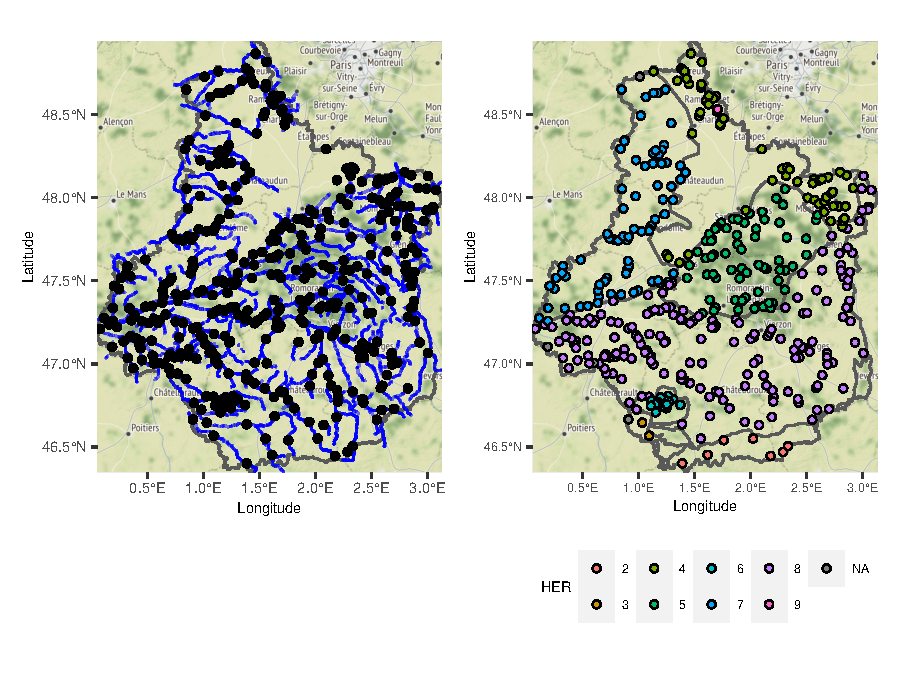
\includegraphics{Chap3/ESU_EX.pdf}
    \caption{Stations monitoring surface waters in the Centre-Val de Loire French region. Two different geographical resolutions are represented. The underlying hydrographic network linking all stations is plotted on the left, the stations are coloured according to their hydro-ecoregion on the right.}
    \label{fig:esu_ex}
\end{figure}

However, we mentioned in Section \ref{chp:2:3} that a single station does not provide many measurements. Therefore, in order to derive information from these data, one can work with a different resolution than that of the station. So there is a trade-off to do between the number of data available to make a statistical statement about a spatial area and the accuracy of the spatial resolution. Another interesting level of resolution, briefly mentioned in Section \ref{chp:2:2}, is defined by the hydro-ecoregions (HER). These are geographical units in which hydrographic ecosystems share common characteristics. The criteria by which they are delineated combine features of geology, terrain and climate \cite{wasson:hal-02580774}. The INRAE services provide such information. Pooling all the samples from the HERs may provide a satisfactory level of aggregation, but this would be at the expense of spatial resolution. Figure \ref{fig:esu_ex} shows how the stations are distributed in the HER.

\subsection{Air quality}
%especially any information  that can be found
Meteorological data is an important dataset for monitoring air quality, it provides for example information about the wind (wind direction, wind strength, etc.). Historical weather records are now available as open data on the Météo France \cite{SYNOP} website. Figure \ref{fig:air_ex} illustrates the cross-referencing of data from air quality monitoring stations with meteorological data. Note that in this example we have chosen stations within the study region, but information from remote areas can also provide interesting information about air pollution in the selected area. This example also shows that concentration monitoring tasks depend on the application context. The coherence of each dataset included in the analysis needs to be discussed.

\begin{figure}[ht]
    \centering
    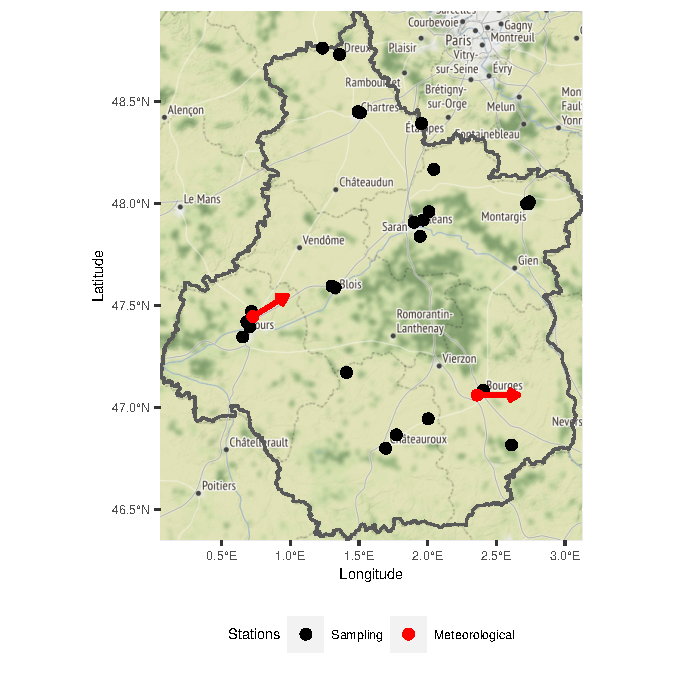
\includegraphics{Chap3/AIR_EX_DATA.pdf}
    \caption{All active stations measuring air quality on March the 1st of 2021 coupled with meteorological stations active that day. The main wind direction and speed measured that day is mapped with the red arrows.}
    \label{fig:air_ex}
\end{figure}

\section{Surveillance of pesticides data}\label{chp:2:5}

This section presents a first exploratory approach to monitoring pesticide concentrations using data from Sections \ref{chp:2:3} and \ref{chp:2:4}. The spatio-temporal nature of concentration data requires appropriate techniques for their representation, which were reviewed in \cite{Andrienko2003,cressie2015,Maimon2010}. This includes the development of visualisation tools. There are several methods for visualising spatio-temporal data, but as mentioned in \cite{Ansari2019}, spatial and temporal resolution is a key factor in the analysis and cannot be chosen automatically. Performing proper analysis of concentration data requires the involvement of experts. In this section, some visualisation techniques are presented and their limitations are discussed. 

The spatial map plots or iterative maps \citep{Andrienko2003} are an effective method to extract information from these data. They consist of maps of the same phenomenon at different times, as in Figure \ref{fig:spa_ex}. There is a clear seasonal pattern in this figure. We can conclude that prosulfocarb is applied in autumn, and this information is affirmed by the crops targeted by this substance, namely winter wheat crops. The two years of observation were segmented by the choice of temporal resolution of the seasons. Although this is a coherent choice, it has some limitations. For example, it cannot take into account years when the treatment started earlier or later due to climatic conditions. In addition, it cannot help to determine precisely the nature of the temporal change in the signal. Only the summarised indicator of quantification rate is used. Nothing is known about the maximum or average concentrations.
 
\begin{figure}[ht]
    \centering
    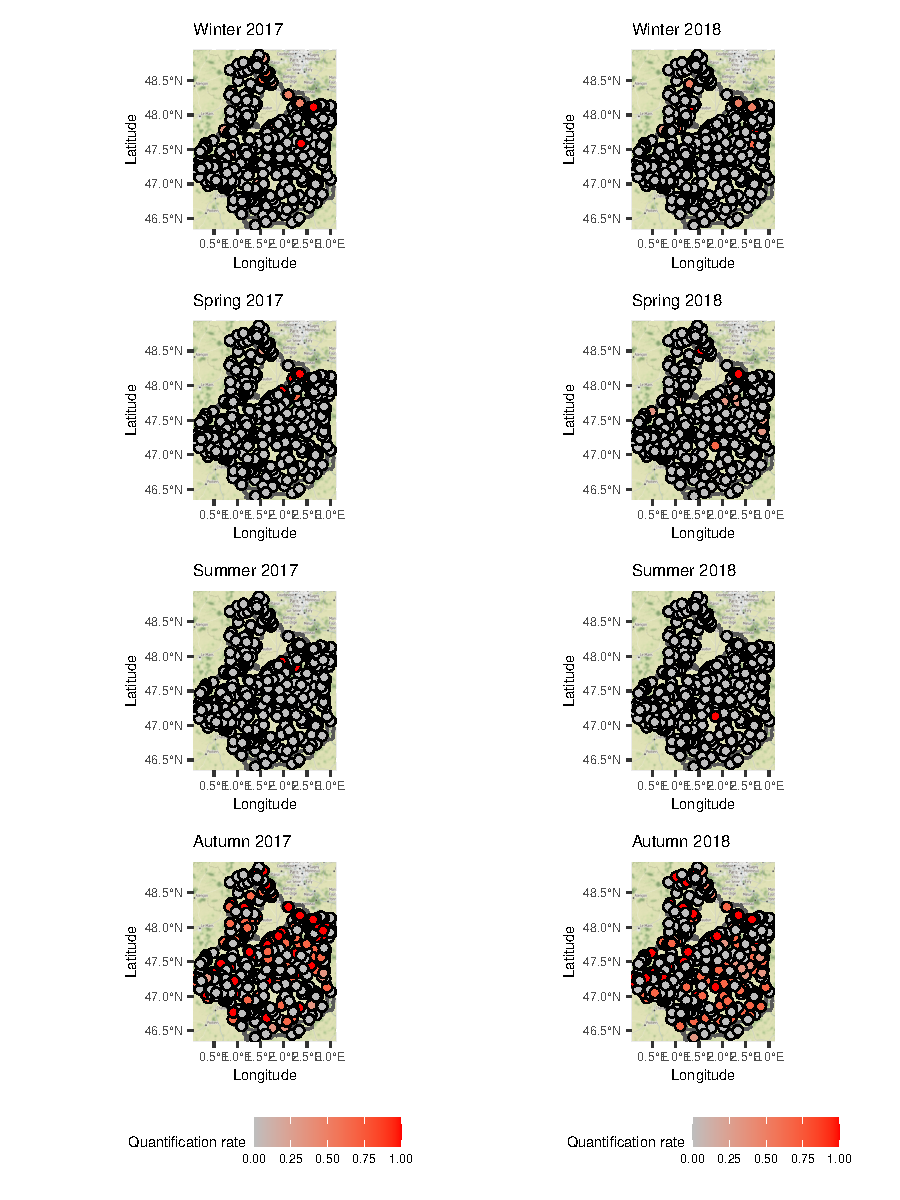
\includegraphics{Chap3/Spatial_maps.pdf}
    \caption{Spatial maps in time. Prosulfocarbe's quantification rate of each station was computed for each season of 2017 and 2018.}
    \label{fig:spa_ex}
\end{figure}

Another conventional representation is to display information with a map animation \citep{Andrienko2003}. In this method, the information displayed on the computer screen is updated according to the selected spatial area. Figure \ref{fig:tsplot_ex} shows a practical example of this technique. The concentrations of prosulfocarbe in the French region Centre-Val de Loire are displayed according to the selected HER region. There are two limitations to this display. The first one is the choice of spatial resolution. The HER were chosen to cluster the geography of the region. However, it can be seen that these can be very large regions. Stations located at opposite corners of a single HER may not have similar concentration values. Spatial heterogeneity of agricultural practises may occur at finer resolution. HER may not accurately capture regions where concentrations are homogeneously distributed. We will show how we deal with the spatial resolution issue in Chapter \ref{chp:5}. This presentation also raises the question of the choice of temporal resolution. All samples available in the studied period are shown in Figure \ref{fig:tsplot_ex}. There is a clear break in the three series around 2015. There seems to be a change in the concentration regimes. \\

In this last example, a finer temporal resolution combined with a comparison of the selected spatial regions could help experts to better understand the evolution of concentrations in the region. The aim of this thesis is to develop a statistical method that helps in the choice of both temporal and spatial resolution and also performs a comparison of the geographical regions at a given time.

\begin{figure}[ht]
    \centering
    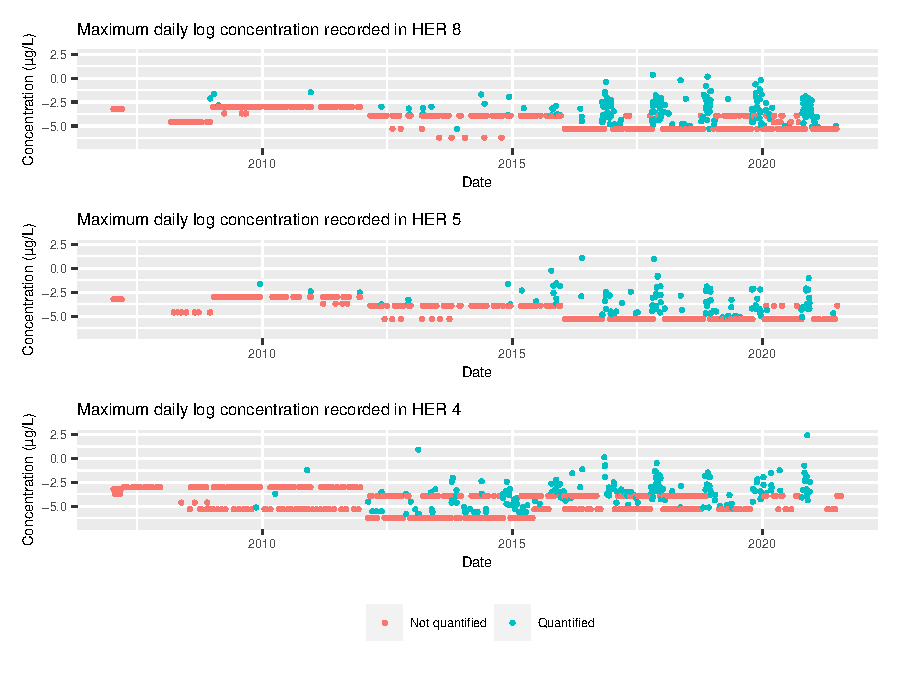
\includegraphics{Chap3/TS_plot.pdf}
    \caption{Time series plot of HER 8,5 and 4 daily maximum concentrations. The log scale was used for a easier visualization.}
    \label{fig:tsplot_ex}
\end{figure}

\clearpage

\section{Chapter summary}

This chapter describes the tasks of the ANSES and the means by which it can fulfil them. The focus is on the task of phytopharmacovigilance. This is a system for monitoring pesticide concentrations and possible adverse effects on living organisms and the environment. The data needed to obtain information on such phenomena are not collected directly by the Agency, but are provided by various administrative departments. Chemical concentration data are subject to specific characteristics such as censoring due to the accuracy of the measuring instruments, spatial and temporal heterogeneity of sampling due to the specificities of the French monitoring network, or spatial and temporal heterogeneity of concentration values explained by the different agricultural practises throughout the territory. Other datasets can be consulted to get a better understanding of the concentration levels and the distribution of the substances. In practice, one way to monitor substances is to combine all these sources of information. Some monitoring tools use visualisation techniques based on these data sets. Although each visualisation technique makes it possible to obtain results in the monitoring mission, it also has disadvantages. We therefore propose to combine visualisation and modelling to improve the monitoring of substances. 

First, the global spatio-temporal heterogeneity of the concentration data must be remedied by searching for homogeneous time periods and geographical areas. We will first focus on the search for homogeneity in the temporal aspect. In Chapter \ref{chp:3} we review the literature to find suitable methods for this task. We then adapt these methods to the specifics of the concentration data in Chapter \ref{chp:4}. Once the method is selected, in Chapter \ref{chp:5} we describe a procedure to deal with spatial heterogeneity and identify abnormal signals of concentration. In Chapter \ref{chp:6} we present a monitoring tool that combines the statistical inference and visualisation method.  



%The minimum number of dimensions to describe them is three: two for space as a pair of longitudes and latitudes; one for time. \cite{cressie2015} presents in his book several methods of descriptive statistics for the representation of such data. The most intuitive method to plot spatiotemporal data are marginal and conditional plot. There are several ways to make them.

 
%\begin{figure}[ht]
%    \centering
%    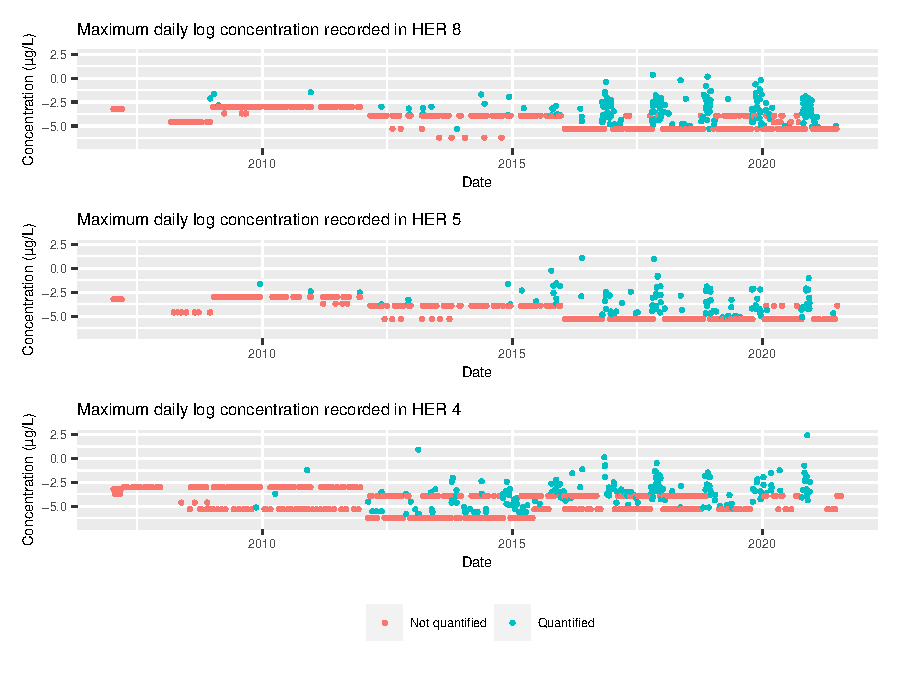
\includegraphics{Chap3/TS_plot.pdf}
%    \caption{Time series plot of HER 8,5 and 4 daily maximum concentrations. The log scale was used for a easier visualization.}
%    \label{fig:tsplot_ex}
%\end{figure}
 


%Another example of representation is the \textbf{space (1-D)/time plots} shown in Figure \ref{fig:S1Dplot}. It consists in fixing a dimension in space whether longitude or latitude and to plot some indicators summarised on that dimension against time. In Figure \ref{fig:S1Dplot}, the longitude was cut into regular intervals and time was segmented in seasons. The plot shows once again a very clear temporal seasons that appears in time in the region. The location of those changes are not clearly displayed by those plots though. We are not able to determine if the large quantification rates are in the central areas of the region or not (given that we miss the latitude information). Although those plots provide an excellent first overview and can help to quickly understand the structure under spatiotemporal data, it does not provide sufficient precision to localize in space and time some interesting signals.    

%\begin{figure}[ht]
%    \centering
%    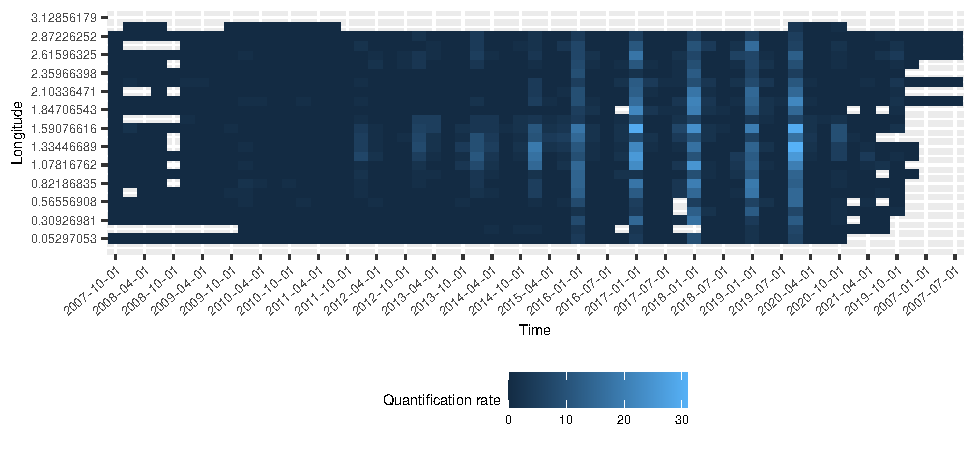
\includegraphics{Chap3/T1Dplot.pdf}
%    \caption{Space (1-D)/Time plots. Grey tiles correspond to location and moment were no sample were collected.}
%    \label{fig:S1Dplot}
%\end{figure}

%All of those representation methods can't capture all the information carried by the data set. We propose to handle it in a dynamic way using the application environment R-shiny. Integrating dynamic response to a user's requests is an efficient way to combine a descriptive view with models results. The application overview will be given in section 6.